\documentclass[12pt]{article}
\usepackage{tikz}
\usepackage{ifthen}
\usetikzlibrary{arrows}

% type, redundancy, required, lambda 
\newcommand{\modelgraphlabel}[4]{$#1$ \\ $r=#2$ \\ $\nu=#3$ \\ $\lambda=#4$}

\begin{document}
% Cloud Model 
\begin{figure}
	% draw - outline, fill - color!alpha, align - allows for manual line-break
	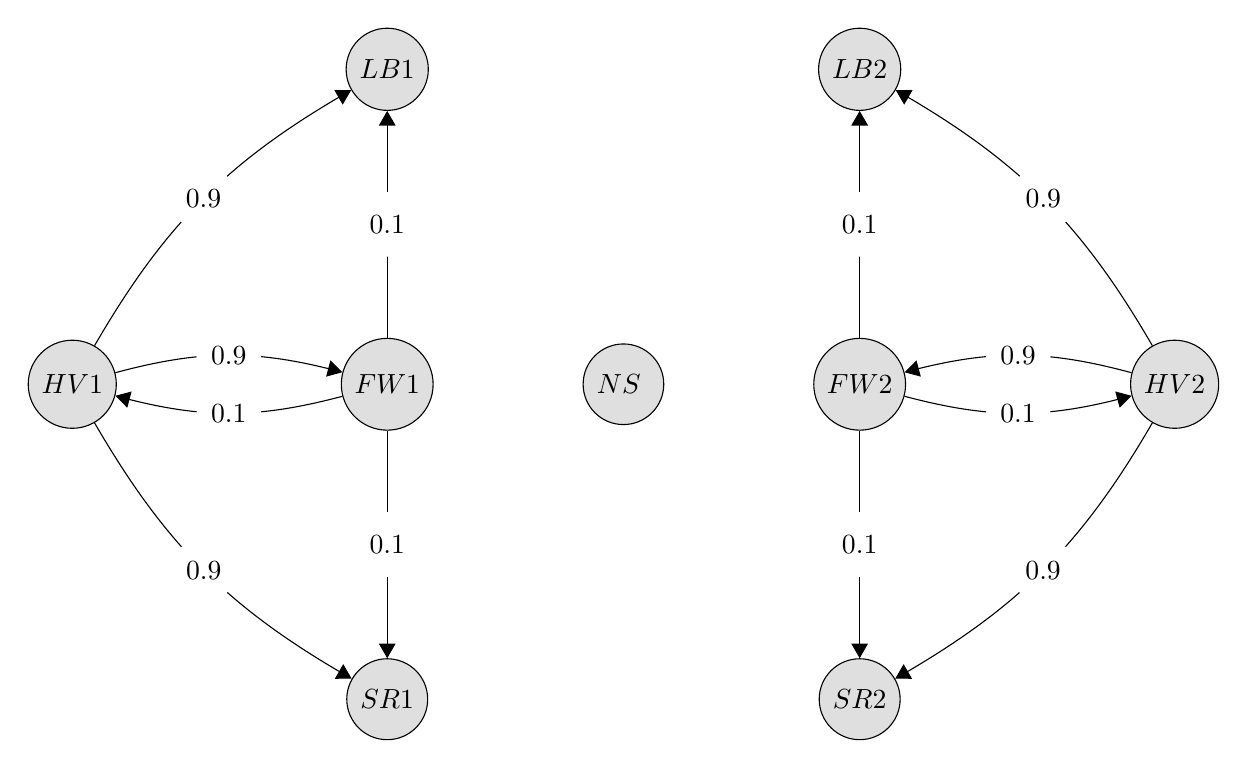
\begin{tikzpicture}[scale = 1, auto = center, every node/.style = {circle,
	draw = black, fill = gray!25}, bend angle = 90]

		\node ($NS$)  at ( 0,  8) [align = center] {{$NS$} };
		\node ($LB1$) at (-3, 12) [align = center] {{$LB1$}};
		\node ($LB2$) at ( 3, 12) [align = center] {{$LB2$}};
		\node ($FW1$) at (-3,  8) [align = center] {{$FW1$}};  
		\node ($FW2$) at ( 3,  8) [align = center] {{$FW2$}};
		\node ($HV1$) at (-7,  8) [align = center] {{$HV1$}};
		\node ($HV2$) at ( 7,  8) [align = center] {{$HV2$}};  
		\node ($SR1$) at (-3,  4) [align = center] {{$SR1$}};
		\node ($SR2$) at ( 3,  4) [align = center] {{$SR2$}};

	    \foreach \from/\phy/\to in {$HV1$/0.9/$LB1$, $HV2$/0.9/$SR2$, $HV1$/0.9/$FW1$, $FW1$/0.1/$HV1$}
	    	\path (\from) edge [-triangle 60, bend left = 15] node[fill=white, draw=none] {\phy} (\to);
	    
	    \foreach \from/\phy/\to in {$HV2$/0.9/$LB2$, $HV1$/0.9/$SR1$, $FW2$/0.1/$HV2$, $HV2$/0.9/$FW2$}
	    	\path (\from) edge [-triangle 60, bend right = 15] node[fill=white, draw=none] {\phy} (\to);
	    
	    \foreach \from/\phy/\to in {$FW1$/0.1/$SR1$, $FW2$/0.1/$SR2$, $FW1$/0.1/$LB1$, $FW2$/0.1/$LB2$}
	    	\path (\from) edge [-triangle 60] node[fill=white, draw=none] {\phy} (\to);
	
	\end{tikzpicture}
	\caption{Cloud-computing architecture}
    \label{fig:cloud}
\end{figure}

\newpage

We now consider a model depicting a cloud-computing architecture shown in
Fig.~\ref{fig:cloud}. There is a directed edge from component type $i$ to
component type $j$ if $j \in \Gamma_i$, and the label on the edge is
$\phi_{i,j}$. $NS$ represents a network switch; $LB1$ and $LB2$ are two types
of load balancers; $FW1$ and $FW2$ denote two types of firewalls; $HV1$ and
$HV2$ signify two types of hypervisors; and $SR1$ and $SR2$ are two types of
server racks. The two types mean different components in the sense that we use
in the paper, i.e., they can be the same model of component but they are
different types because they are in different parts of the system. This
organization of components specifically shows a firewall ``sandwich" as
described in \cite{Godd:2001}.

We set $r_{NS} = r_{LB1} = r_{LB2} = r_{FW1} = r_{FW2} = r_{HV1} = r_{HV2} =
2$ and $r_{SR1} = r_{SR2} = 3$. We assume the system is operational if at
least $\upsilon_i$ components of each type $i$ are up. We need at least two
server racks of each type $SR1$ and $SR2$ to be up to be able to parallel
process across server racks. For other component types, we require at least
one component of each type of the system to be up for the system to remain
operational. Thus, $\upsilon_{SR1} = \upsilon_{SR2} = 2$ and $\upsilon_{NS} =
\upsilon_{LB1} = \upsilon_{LB2} = \upsilon_{FW1} = \upsilon_{FW2} =
\upsilon_{HV1} = \upsilon_{HV2} = 1$. Additionally, our system operates in two
environments: high demand ($e = 0$) and low demand ($e = 1$). This gives us a
state space of size 69984. Solving this using the previous version of DECaF
takes xxx seconds, whereas using the new version takes xxx seconds.

We work with a system such that all component types that are located to the
left of $NS$ (i.e., types with a ``1" in their names) handle SMTP requests
only, whereas all component types located to the right of $NS$ (i.e., types
with a ``2" in their names) handle HTTP requests only. Thus, both groups of
components (i.e., to the left and to the right of $NS$) need to be operational
for the system to be able to handle HTTP and SMTP requests. The decoupling
ensures that hardware failure on one side does not immediately propagate to
the other.

As stated in \cite{ReHype:2011}, ``hypervisors almost always cause other
system components to fail and certainly cause server racks to fail because of
state corruption." Thus, we assume $\phi_{HVi,LBi} = \phi_{HVi,FWi} =
\phi_{HVi,SRi} = 0.9$ for $i = 1, 2$. We also assume $\phi_{FWi,LBi} = 
\phi_{FWi,HVi} = \phi_{FWi,SRi} = 0.1$ for $i = 1, 2$.

To estimate the component failure rates, we assume that in a high-demand
(resp., low-demand) environment, a hardware component is going to fail
on average in twice (resp., eight times) the time of its warranty. The time unit
is hours. Typical commercial network switches, load balancers and hypervisors
have warranties of 90 days (2160 hours). Thus, $\lambda_{NS, \, 0} =
\lambda_{LB1, \, 0} = \lambda_{LB2, \, 0} = \lambda_{HV1, \, 0} =
\lambda_{HV2, \, 0} = 1 / 4320$ and $\lambda_{NS, \, 1} = \lambda_{LB1, \, 1}
= \lambda_{LB2, \, 1} = \lambda_{HV1, \, 1} = \lambda_{HV2, \, 1} = 1 /
17280$. Commercial server racks often have 3-year warranties giving us
$\lambda_{SR1,\, 0} = \lambda_{SR2, \, 0} = 1 / 52560$ and $\lambda_{SR1, \,
1} = \lambda_{SR2, \, 1} = 1 / 210240$. Since firewalls fail due to numerous
reasons such as software bugs or from targeted attacks, it is difficult to
find a single representative failure rate. Thus we assume a software firewall
fails on average once in five years, and set $\lambda_{FW1, 0} =
\lambda_{FW2, 0} = \lambda_{FW2, 1} = \lambda_{FW1, 1} = 1 / 43800$.

As given in \cite{Godd:2001}, failed hardware components are repaired with a
rate of $1 / 24$ regardless of the environment, i.e., we can replace one component
a day on average. Firewalls being non-hardware components need to be rebooted
after they fail, and this occurs with a rate of 10, which is also taken from
\cite{Godd:2001}. The environment switches once every 12 hours on average,
giving us the environment transition rates $\nu_{0, 1} = \nu_{1, 0} = 1 / 12$.

\bibliographystyle{plain}
\bibliography{cloud}

\end{document}